\subsection{Beta version}
\label{kap:McpExecutorBetaversion}
Für die Betaversion der Mcp-Executor-Einheit werden alle Komponenten in ein Gehäuse integriert (s. Abbildung \ref{fig:McpExecutorBeta}), welches gerade so groß ist, dass es beim Tragen am Körper möglichst nicht stört und einfach befestigt werden kann. Für das Integrieren werden zusätliche Platinen angefertigt.
\newline
Aufgrund des Feststellens verschiedener negativer Aspekte während der Entstehung der EInheiten existieren mehrere Beta-Versionen.

\begin{figure}[H]
	\centering
	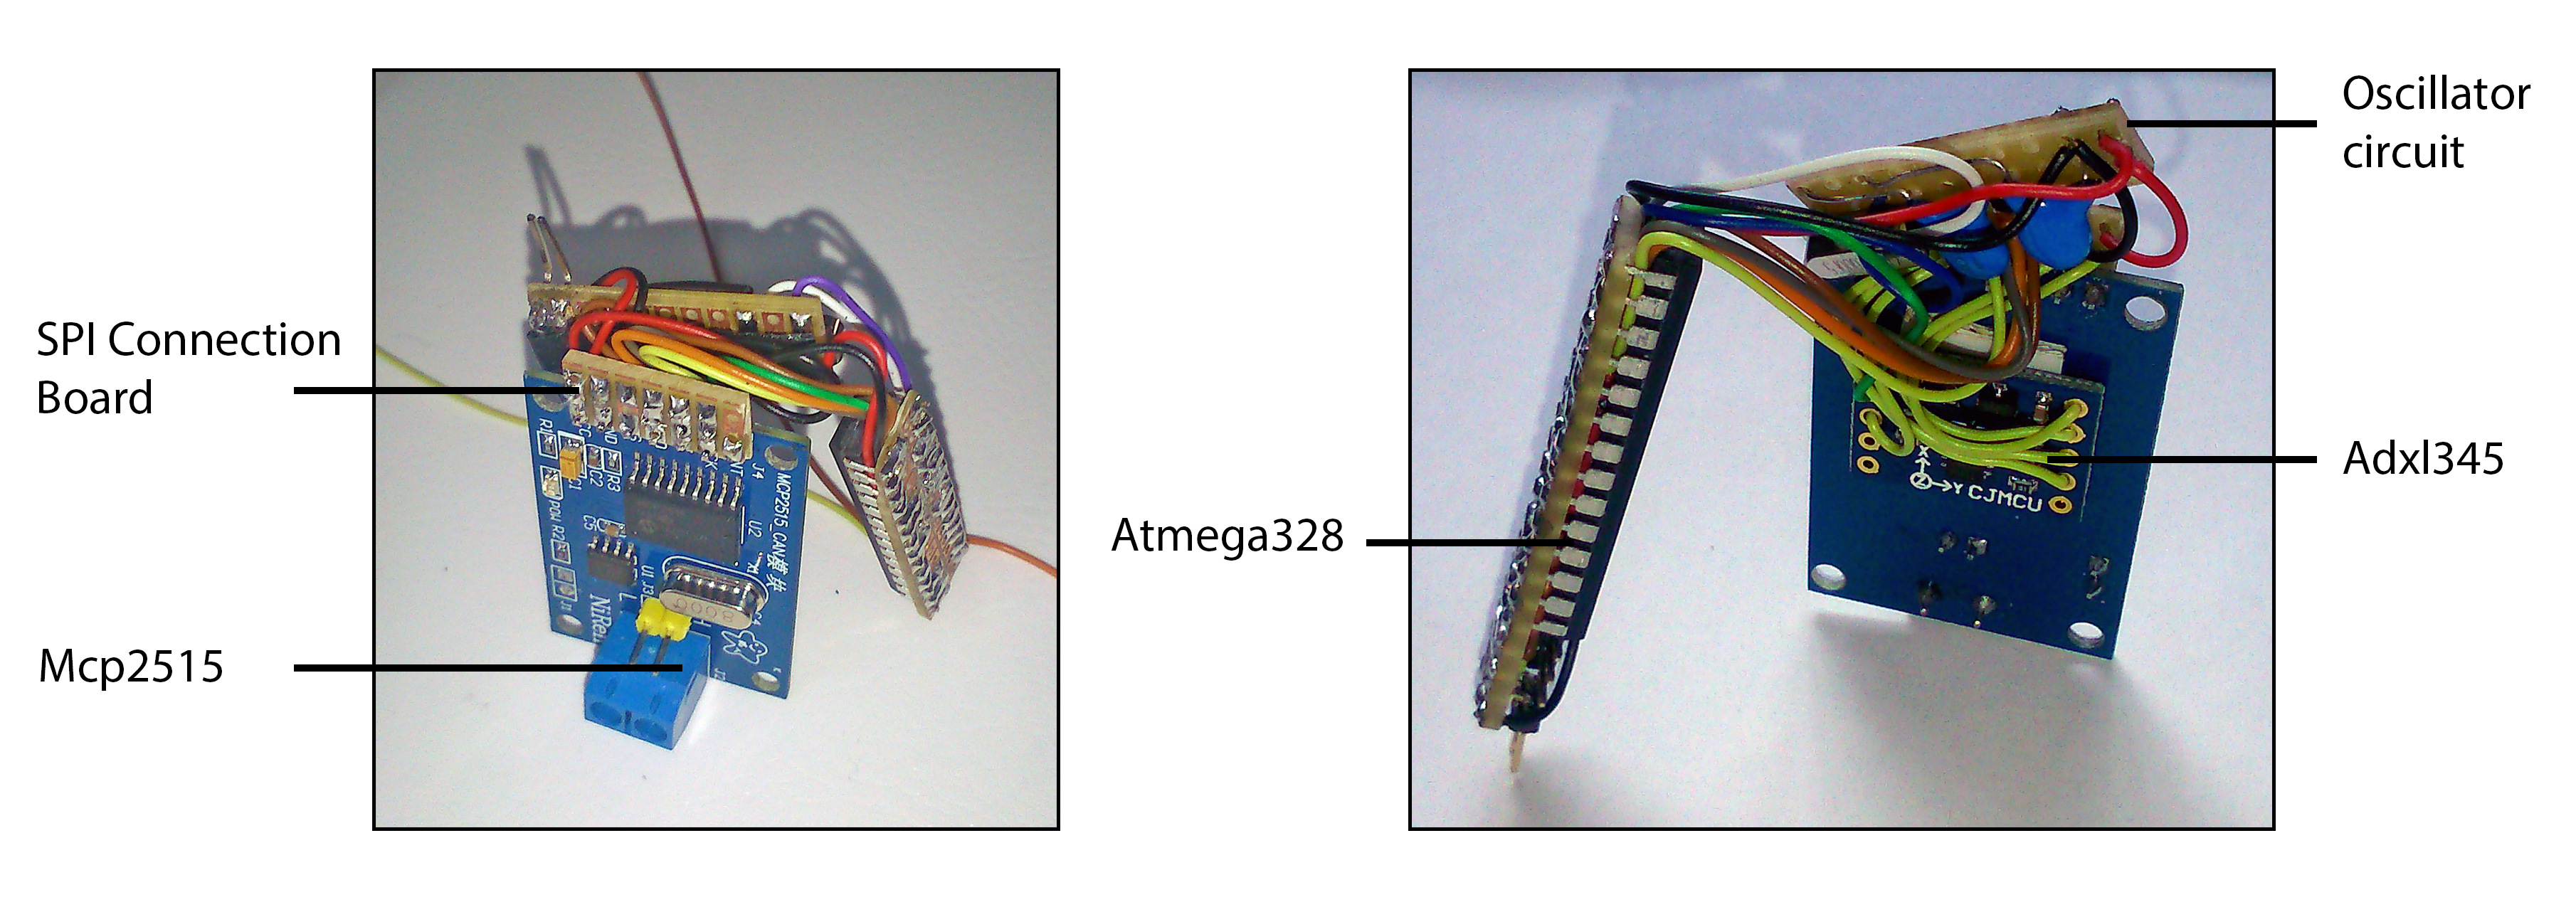
\includegraphics[width=1.0\linewidth]{Bilder/McpExecutor_BetaDetail}
	\caption[Betaversion einer Mcp-Executor-Einheit]{Betaversion einer Mcp-Executor-Einheit}
	\label{fig:McpExecutorBeta}
\end{figure}

Die Befestigung der Einheit am Körper erfolgt anhand eines Positioniergurtes. Dieser besteht in der ersten Beta-Version aus zwei und in der zweiten Version aus einem Klettverschluss, die an dem Abdeckblech der Einheit befestigt sind. Durch ein entsprechendes Gegenstück des Klettverschlusses auf der Rückseite des Abdeckblechs ist der notwendig Halt gegeben.
%
% BILD KLETTVERSCHLUSS
%
\begin{figure}[H]
	\centering
	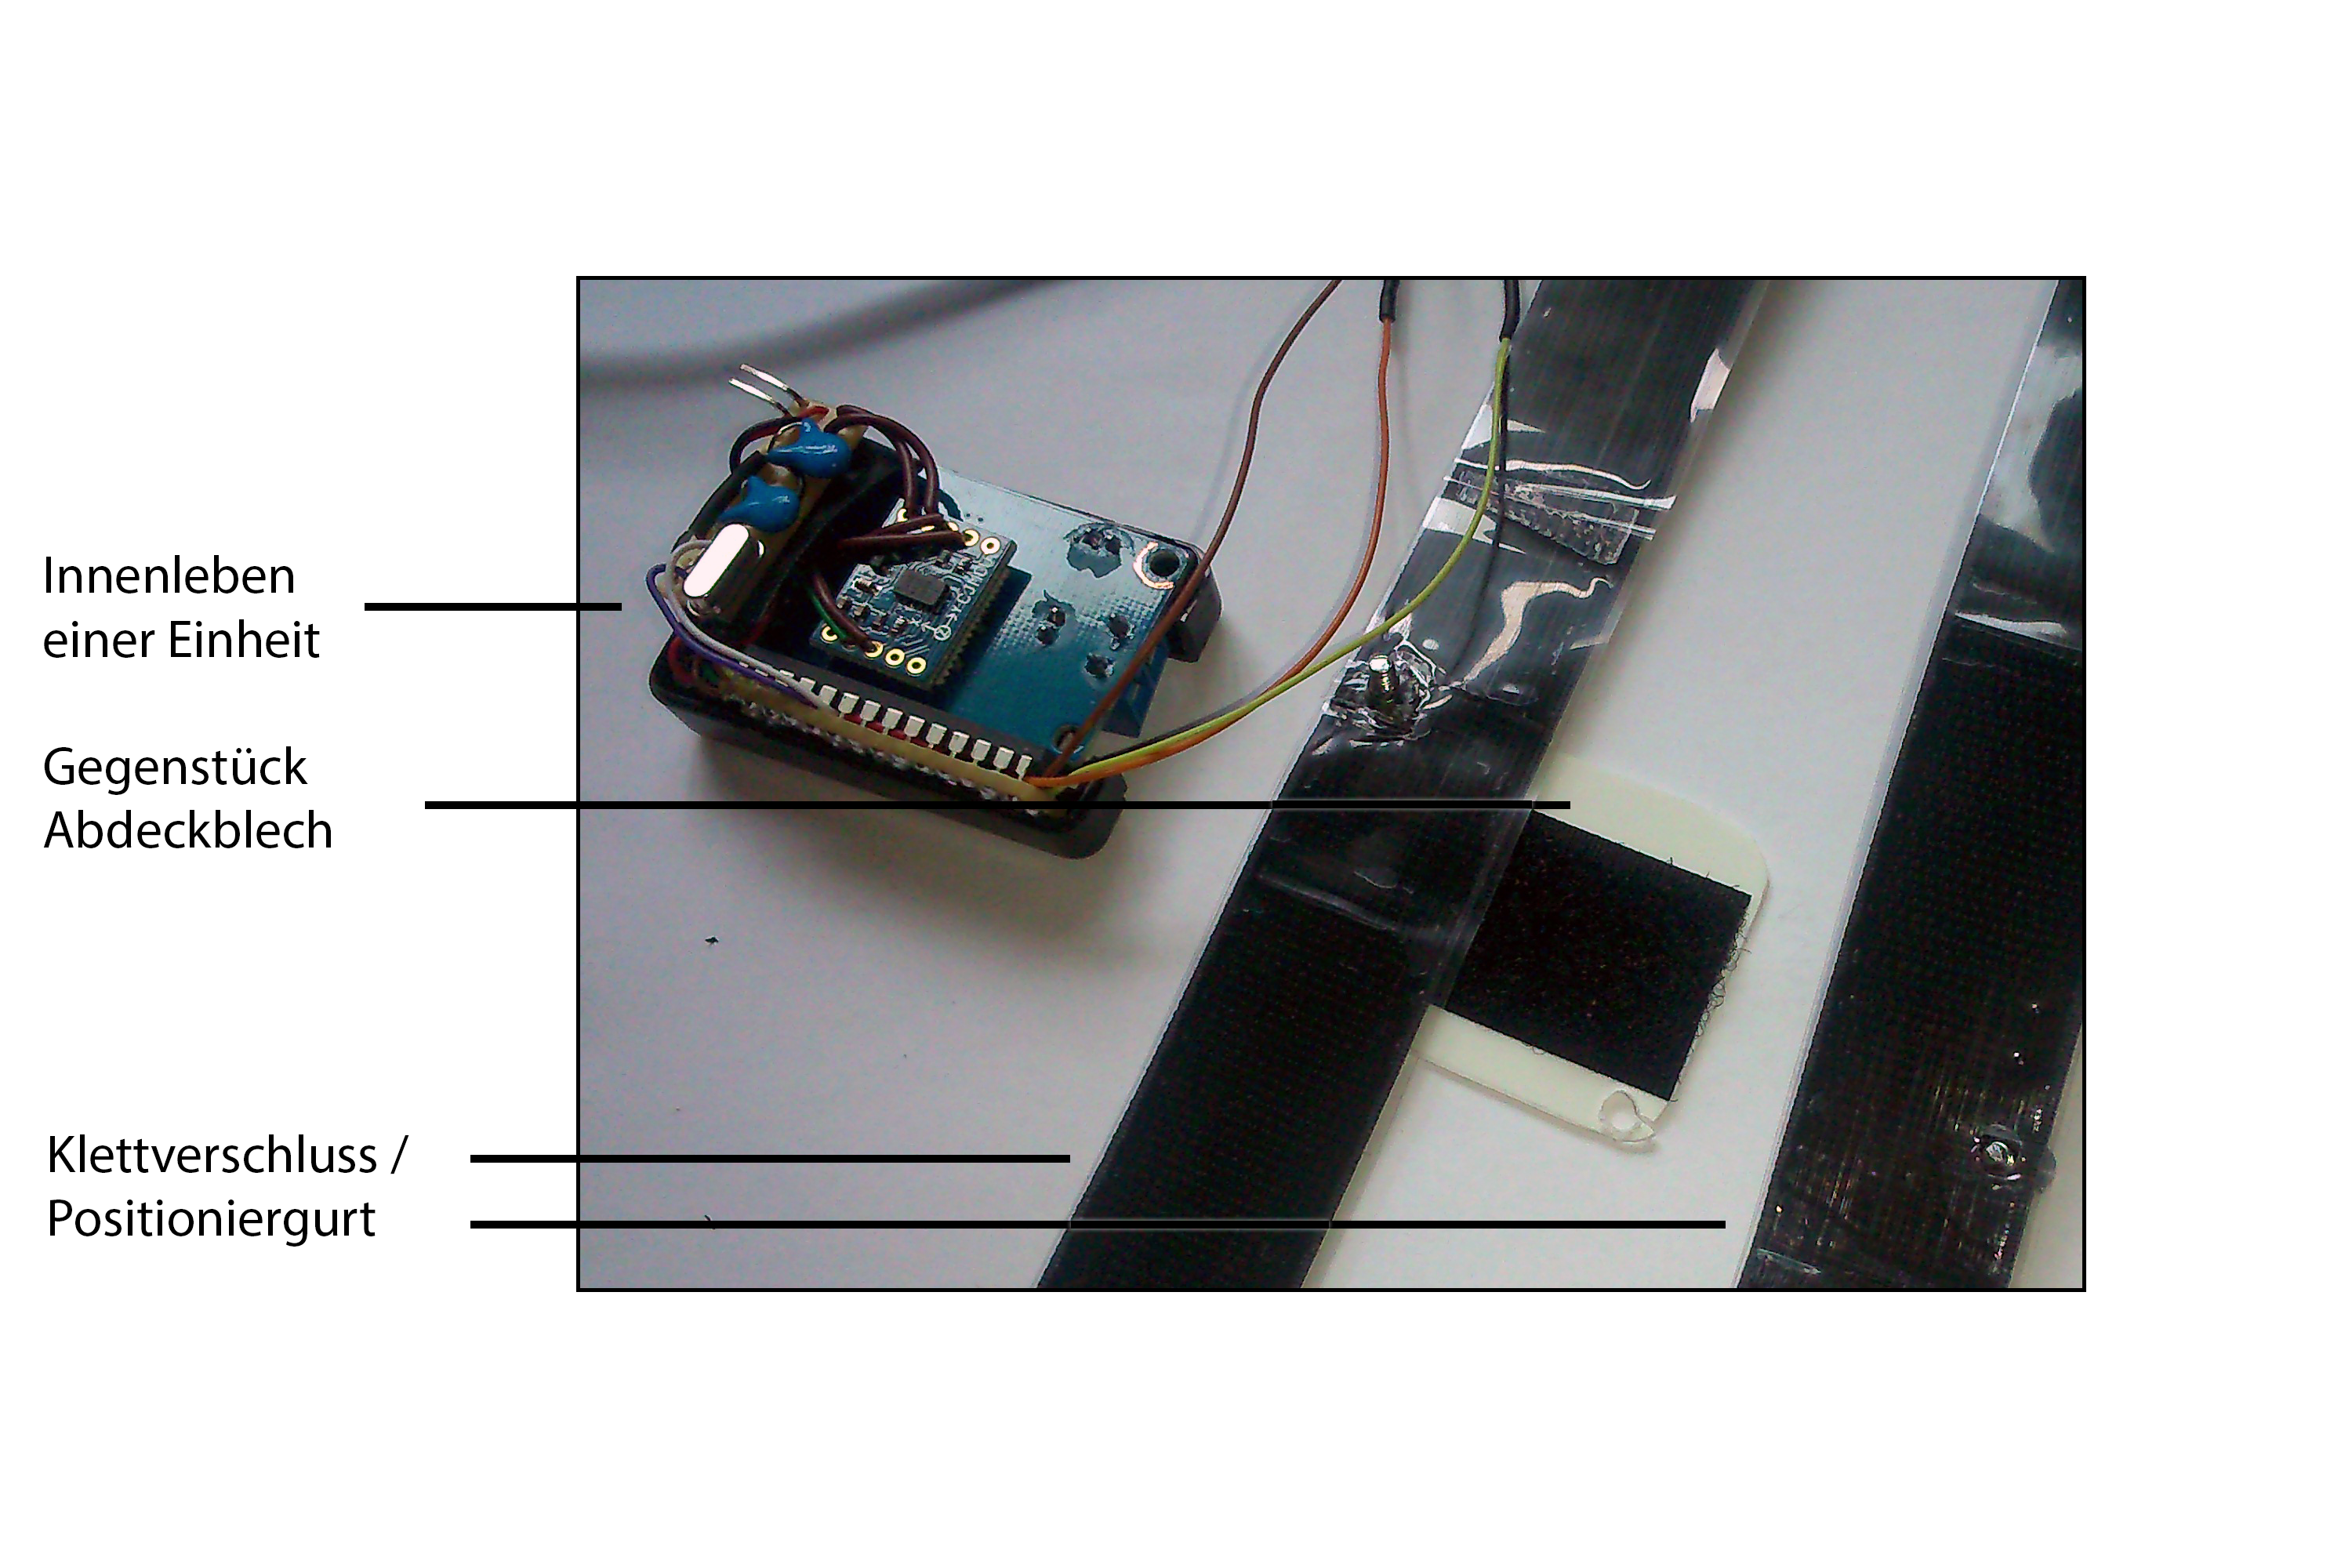
\includegraphics[width=1.0\linewidth]{Bilder/McpExecutor2515Klettverschluss}
	\caption[Betaversion einer Mcp-Executor-Einheit - Klettverschluss]{Betaversion einer Mcp-Executor-Einheit - Klettverschluss}
	\label{fig:McpExecutorBetaKlettverschluss}
\end{figure}

An dem Anzug sind ebenfalls entsprechende Gegenstücke des Klettverschlusses angebracht, sodass die Einheiten während der Bewegung nicht verrutschen. 

